\documentclass[border=6pt]{standalone}
\usepackage{tikz}
\begin{document}
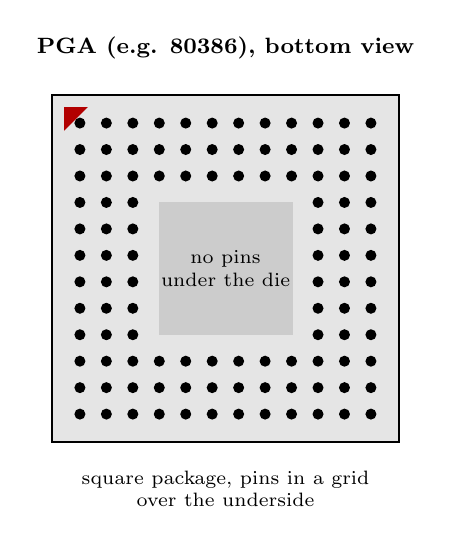
\begin{tikzpicture}[font=\small]
% PGA bottom view
\begin{scope}
\node[font=\footnotesize\bfseries] at (2.2,5.0) {PGA (e.g. 80386), bottom view};
\draw[thick,fill=gray!20] (0,0) rectangle (4.4,4.4);
\fill[gray!40] (1.35,1.35) rectangle (3.05,3.05);
\node[font=\scriptsize,align=center] at (2.2,2.2) {no pins\\under the die};
\foreach \i in {0,...,11} \foreach \j in {0,...,11} {
  \pgfmathsetmacro{\x}{0.35+0.336*\i}
  \pgfmathsetmacro{\y}{0.35+0.336*\j}
  \pgfmathtruncatemacro{\inner}{(\i>2)*(\i<9)*(\j>2)*(\j<9)}
  \ifnum\inner=0 \fill (\x,\y) circle (0.07); \fi
}
\fill[red!70!black] (0.15,4.25) -- (0.45,4.25) -- (0.15,3.95) -- cycle;
\node[font=\scriptsize,align=center] at (2.2,-0.6) {square package, pins in a grid\\over the underside};
\end{scope}
\end{tikzpicture}
\end{document}
